\documentclass[12pt, a4paper]{article}
\usepackage[utf8]{inputenc}
\usepackage{natbib}
\usepackage[french]{babel}
\usepackage[T1]{fontenc}
\usepackage{graphicx}
\usepackage{fancyhdr}
\usepackage{lastpage}
\usepackage[margin=2cm, headheight=2cm]{geometry}
\pagestyle{fancy}
\usepackage{hyperref}
\fancyhf{}
\lhead{Prénom Nom}
\chead{Compte rendu hebdomadaire du mercredi 15 juillet 2020}
\rhead{\thepage / \pageref{LastPage}}
\AtBeginDocument{\def\labelitemi{$\bullet$}} % textbullet textendash textasteriskcentered textperiodcentered blacksquare square bullet circ
\AtBeginDocument{\def\labelitemii{$\circ$}}
\begin{document}
\section{Travaux effectués}

\begin{itemize}
\item Description tâche 1 avec comme sous-tâches:
	\begin{enumerate}
	\item Sous-tâche 1
	\item Sous-tâche 2	
	\end{enumerate}
\item Description tâche 2 avec l'\autoref{eq:deconvolution}

\begin{equation}
    \label{eq:deconvolution}
    h(n) = IFFT \left( \frac{FFT(y(n))}{FFT(x(n))} \right)
\end{equation}

\end{itemize}

\section{Travaux en cours}

\begin{itemize}
\item Description tâche 1 en lien avec la \autoref{fig:orosys}

\begin{figure}[h!]
\centering
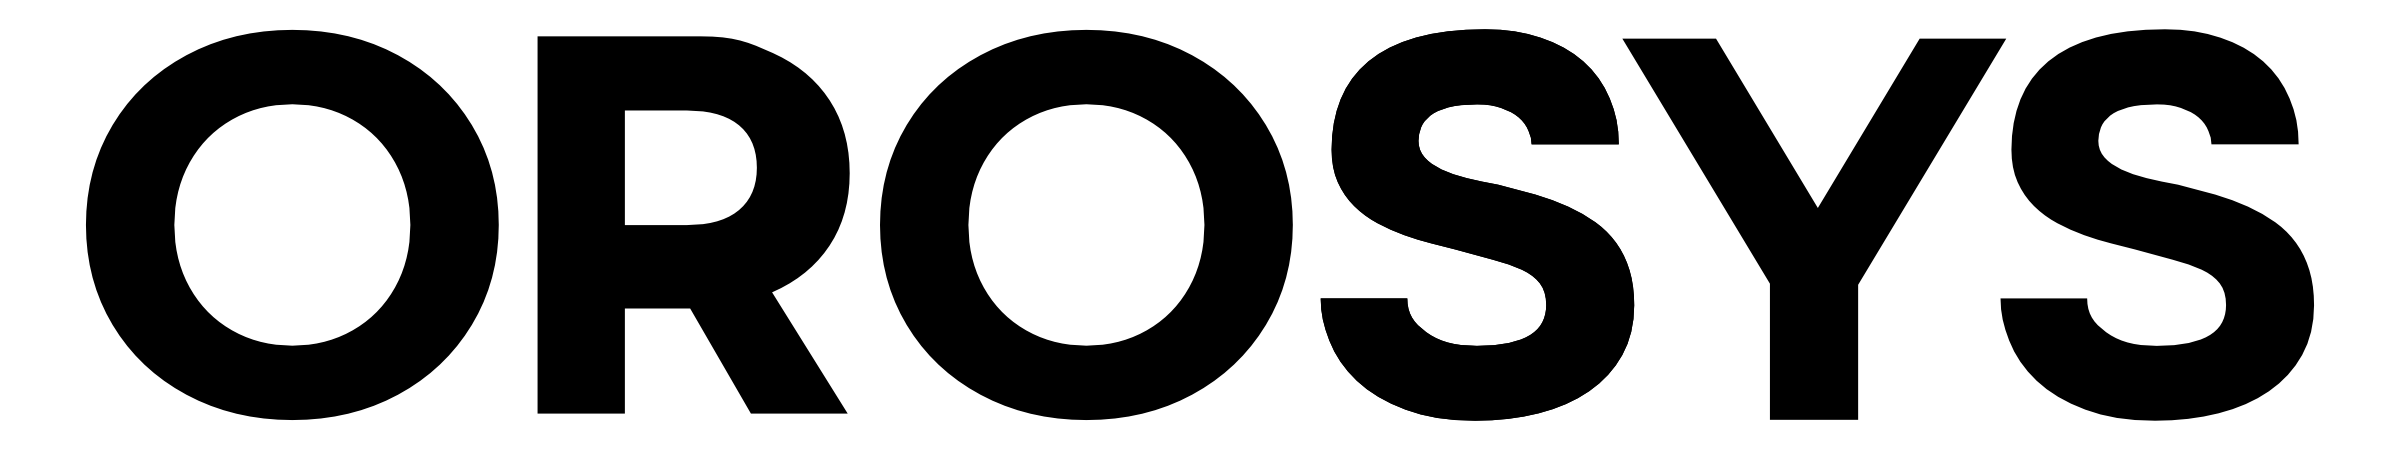
\includegraphics[width=\linewidth]{orosys.png}
\caption{Exemple de titre de figure}
\label{fig:orosys}
\end{figure}

\item Description tâche 2 comme dans \url{https://www.two-notes.com/fr}

\end{itemize}

\section{Travaux à réaliser}

\begin{itemize}
\item Description tâche 1 en lien avec le \autoref{table:performances}

\begin{table}[!h]
    \centering
    \caption{Exemple de titre de tableau}
    \label{table:performances}
    \begin{tabular}{c|ccc}
                 &      \multicolumn{3}{c}{(x,y)}            \\
        Position &       cm     &      \%       &   Float     \\
        \hline
        A        & ( 0 cm,  0 cm) & (  0\%,  0\%) & (0.0,0.0)   \\
        B        & (13 cm,  0 cm) & (100\%,  0\%) & (1.0,0.0)   \\
        C        & ( 0 cm,240 cm) & (  0\%,100\%) & (0.0,1.0)   \\
        D        & (80 cm,240 cm) & (100\%,100\%) & (1.0,1.0)   \\
    \end{tabular}
\end{table}

\item Description tâche 2 comme \citep{Zhang2018LSTM}
\end{itemize}

\bibliographystyle{plainnat}
\bibliography{references}
\end{document}
